\section{Wstęp}
%%%%%%%%%%%%%%%%%%%%%%%%%
	\begin{frame}{Wstęp} 
		\textcolor{blue}{Problem:}

		\begin{itemize}
			\item Wiele całek nieoznaczonych nie daje się wyrazić w postaci skończonej przez funkcje elementarne
			\item Częsta niemożliwość znalezienia dokładnych całek oznaczonych
    	\end{itemize}

		\textcolor{blue}{Przykłady:}
		\begin{itemize}
			\item $\int_{0}^{2}e^{-x^{2}} dx$
			\item $\int_{0}^{\pi}cos(3cos\theta) d\theta$
    	\end{itemize}
    	
    	\textcolor{blue}{Rozwiązanie:}
    	\begin{itemize}
    	\item Zastąpienie funkcji podcałkowej $f(x)$ inną bliską funkcją $g(x)$, przybliżenie całki przez sumę ważoną:
    	\end{itemize}
    	$$I=\int_{a}^{b}f(x)dx \approx\sum_{i=0}^{n}A_{i}y_{i}$$
   	 	
	\end{frame}
%%%%%%%%%%%%%%%%%%%%%%%%%
	\begin{frame}
    
a) \textit {kwadratura} - przypadek specjalny zagadnienia początkowego\footnote{zagadnienie polegające na znalezieniu konkretnej funkcji spełniającej dane równanie różniczkowe i warunek początkowy.}:
$$
 I=\int_{a}^{b}f(x)dx\ \equiv I=y(b)
$$
\textcolor{blue}{Dane:} 
\begin{itemize}
	\item pochodna: $\displaystyle \frac{dy}{dx}=f(x)$
	\item warunek początkowy: $y(a)=0$
  \end{itemize}
\end{frame}
%%%%%%%%%%%%%%%%%%%%%%%%%	    
    \begin{frame}
    
      b)
      \begin{center}
      	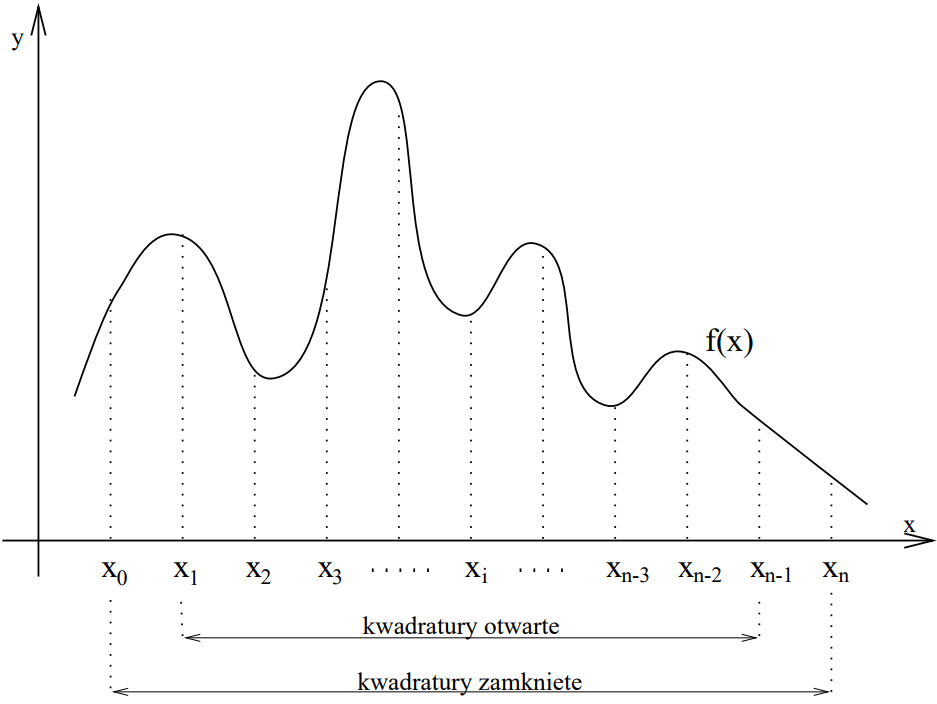
\includegraphics[width=0.6\linewidth]{img/6/image001.png}
      \end{center}
      
      \begin{block}{}
      Kwadratury:
      
        \begin{itemize}
          \item otwarte 
          \item zamknięte
          \item półotwarte
        \end{itemize}
      \end{block}
    \end{frame}
%%%%%%%%%%%%%%%%%%%%%%%%%
    \begin{frame}
    	c) \textbf{Istota}: $\newline$
    	 Podział przedziału całkowania [a,b] na podprzedziały $\rightarrow$ formuły złożone
        $$
	        I=\int_{a}^{b}f(x)dx\ = \sum_{i=0}^{n}\int_{a_{i}}^{a_{i+1}}f(x)dx=\sum_{i=0}^{n}I_{i}
        $$
		d) \textbf{Stopień dokładności kwadratury}: $\newline$
        \textit{E} - błąd kwadratury,$\newline$
         {$P_{k}$} - wielomian stopnia k, $\newline$
        Stopień - liczba całkowita n $>$ 0 :
        $$\forall k\leq n : E(P_{k})=0, \newline
			   E(P_{n+1})\neq 0$$
	
        całkowanie, dodawanie - operacje liniowe $\rightarrow$ zamiast $P_{k}$ $\rightarrow x^{k}.$
    \end{frame}
%%%%%%%%%%%%%%%%%%%%%%%%%
	\begin{frame}{Ekstrapolacja Richardsona}
		Metoda uzyskiwania wyników o dużej dokładności przy użyciu formuł niskiego rzędu.	
		$\newline$
		$\newline$
       Historyczne podejścia:
        \begin{itemize}
          \item Archimedes (200 p.n.e.)
          \item L. F. Richardson, J. A. Gaunt (1927 n.e)
        \end{itemize}
        $\newline$
        Niech	\textit{h} - krok metody, \textit{E(h)} - błąd obliczeń $\rightarrow$ postać asymptotyczna
        $$
			E(h)=\sum_{i=k}^{\infty}a_{i}\cdot h^{i},\ a_{k}\neq 0
		$$
		przy czym: $a_{i}$
         $\left\{\begin{array}{l}
  			\textnormal{mogą zależeć od \textit{f}(x),}\\
            \textnormal{\textbf{nie} zależą od h.}
        \end{array}\right\}$
   \end{frame}
   
   \begin{frame} 
   Obliczenia dla $h_{1}\neq h_{2}:$ $\newline$
   $\varphi$ -- dokładna wartość $\newline$
   $\varphi_{1}, \varphi_{2}$-- wartości wyznaczone
   $\newline\newline$
   Cel $\rightarrow$ zwiększenie minimalnego wykładnika przy h o 1,$\newline\quad$ początek sumowania w (k+1)
		$$
        \begin{array}{l}
\varphi=\varphi_{1}(h_{1})+\sum_{i=k}^{\infty}{a_{i}}\cdot h_{1}^{i}\ \text{\textbar}\cdot h_{2}^{k}\\
\varphi=\varphi_{2}(h_{2})+\sum_{i=k}^{\infty}{a_{i}}\cdot h_{2}^{i}\ \text{\textbar}\cdot h_{1}^{k}
		\end{array}\Bigg\lvert - 
        $$
        
		$$
\varphi=\frac{1}{h_{1}^{k}-h_{2}^{k}}\cdot(h_{1}^{k}\cdot\varphi_{2}-h_{2}^{k}\cdot\varphi_{1})+\sum_{i=k+1}^{\infty}a_{i}\cdot\frac{h_{1}^{k}h_{2}^{i}-h_{1}^{i}h_{2}^{k}}{h_{1}^{k}-h_{2}^{k}}
		$$
		Wynik $\Rightarrow$ zwiększenie najmniejszego wykładnika potęgi \textit{h} w \textit{E(h)} , \\
		ER pozwala poprawić wynik nawet gdy od razu wybrano metodę rzędu \textit{k} + 1.        
	\end{frame}
%%%%%%%%%%%%%%%%%%%%%%%%%
	\begin{frame}
		Szczególny przypadek ER (użyteczny dla kwadratur):
		$$
\varphi=N_{j-1}(h)+\sum_{j=1}^{m-1}K_{j}\cdot h^{2j}+O(h^{2m})\ ,
        $$
        co pozwala na rekurencyjne generowanie:   
        $$
N_{j}(h)=\displaystyle \frac{1}{4^{j-1}-1}\cdot[4^{j-1}\cdot N_{j-1}(\frac{h}{2})-N_{j-1}(h)],\ \ j=2, 3, . . ., m.
		$$
    \end{frame}
%%%%%%%%%%%%%%%%%%%%%%%%%




